\section{Introduction and Background}

% \nsnote{alot of what happens in the Abstract}

% \nsnote{talk about how the gradient is important. how its used}

% \nsnote{talk about how suas are used to collect science data}

The goal of this paper is to investigate the feasibility of using multiple small Uncrewed Aerial Systems (UAS) to cooperatively estimate an unknown wind field. 
If multiple UAS are flying in a formation, algorithms can be implemented to allow the sensor data from each UAS to be fused together to collaboratively estimate a wind field.
The combined estimate of the wind field should be more accurate than a single UAS estimate, as formation flying allows for higher observability of the wind field; taking measurements at different temporal and spacial locations.

Accurate wind field estimation is important for many applications of UAS flight, wind energy extraction, and civil engineering. The ability to cooperatively estimate the wind field would allow small UAS to fly more efficiently, using dynamic soaring to extract energy from the wind.
Accurate wind field estimation is also critical from a science perspective; wind gradient data is critically important for the design of buildings and wind turbines arrays for maximum energy extraction \cite{abdalla2023, matiko2013, rehman2008, vasel2017}. 
Additionally, collabrative estimation allows for more robustness to failures. If one UAS or sensor malfunctions, the wind field estimation is not blocked, but just degraded. 

The current state of the art for wind field estimation is to use CFD simulations over the surface of the terrain to fit the wind gradient to the power law relationship \cite{probst2010}.
These simulations have been proven to perform well for slopes lower than $25\%$ grade. 
But, running CFD simulations is computationally expensive and time consuming. 
The agility of having a fleet of UAS to quickly survey the wind field would allow for faster wind field estimation, although it does require an in-person presence.
However, CFD simulations are way too computationally expensive to be used online in a UAS.
As mentioned above, the ability for a UAS to estimation the wind field online may allow unique explotation of the wind using dynamic and static soaring techniques.


Wind gradients vary drastically depending on weather conditions and terrain. An example of how human made buildings impact the wind gradient is shown in Figure~\ref{fig:wind_gradient_buildings}. 
This figure shows the impact terrain has on the surface roughness, $\alpha$, which is directly proportional to the wind gradient in the boundary layer.
Because of the high variablility of the wind gradient, any usage of UAS for wind field estimation must be robust and able to handle a wide range of wind gradients.

\begin{figure}[h]
    \centering
    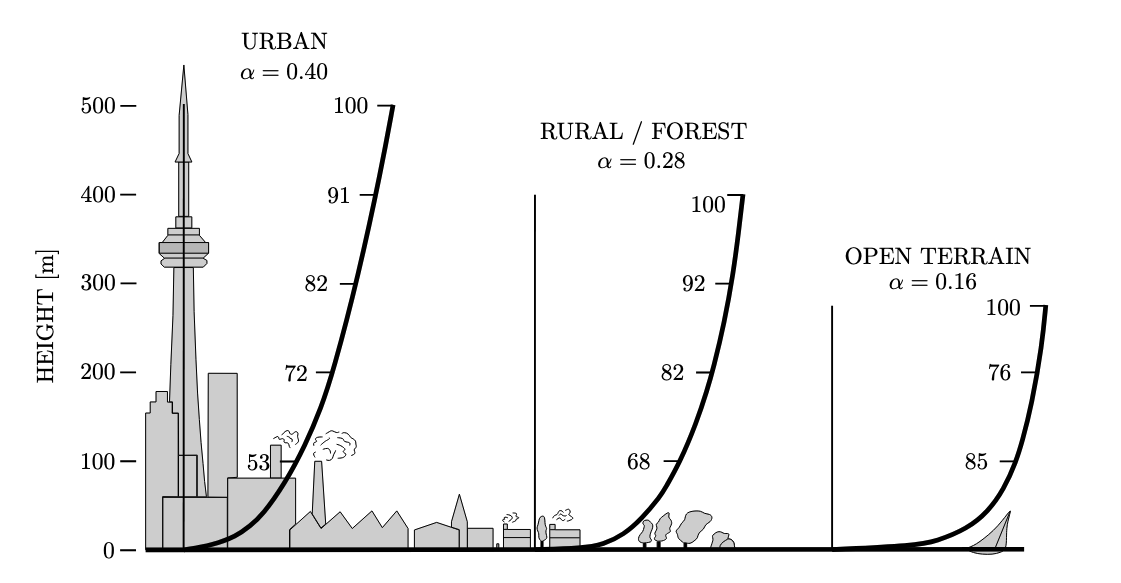
\includegraphics[width=0.5\textwidth]{images/wind_gradient_buildings.png}
    \caption{Impact of terrain on surface roughness, $\alpha$, and wind gradient, \cite{recoskie2017}}
    \label{fig:wind_gradient_buildings}
\end{figure}

This paper will explore using a robust centralized online optimizer to estimate the wind field using a series of wind measurements taken from a formation of UAS.
The pros, cons, and improvements on this approach will be discussed in detail.